\section{Executive Summary}
\iffalse
The purpose of this introduction to your idea is to clearly and succinctly describe the final goal of the project. It should list key features and components and explain why the project is interesting and worthwhile.

When "searching for funding/approval" you have very little time/space to capture the interest of the reader. You need to concisely describe what the project will do, what need it will address, and why a completed project with be of benefit. You also need to convey interest, enthusiasm, and determination. You want the reader coming away from this first page eager to know more and excited about the prospects.
 
This section should be one page long.

NOTES:
Look at: 
"Success in introductory college physics: the role of high school preparation"

"STEM Attrition: College Students' Paths Into and Out of STEM Fields"

"Trends in International Mathematics and Science Study"
via www.aps.org/units/fed/newsletters/aug98/timss2.html
\fi
\BgThispage
Physics is one of the core subjects that college-bound high school students will explore, especially for those that plan to pursue a degree in a scientific field. However, many instructors have doubts about how well high school courses are preparing students for their college experience. In the Third International Mathematics and Science Study (TIMSS), 18 participating countries tested student populations from elementary, middle, and high school on a broad range of physics concepts. The average result was that students were only able to answer 35\% of the questions correctly \cite{TIMSS}. For U.S. students, the average dropped to 24\%.

Clearly, there is a need for improvement in this area. Our team believes that we can provide a web-based solution that would have the power to make a difference both for high school students and for students taking college level physics for the first time. Our project will be called Principia, named after \textit{Philosophiæ Naturalis Principia Mathematica}, the collection of books written by Newton that serves as the foundation of classical mechanics. 

We envision Principia as something that is in equal parts an engaging community experience and a powerful tool to model physical systems. Students will have a support network to help them overcome challenges and a chance to share their knowledge with others. Instructors will have a website they can use to cover material in a deeper and more captivating way than a traditional lecture that uses static images.

The core feature will be an interactive sandbox for designing systems. It will include a toolbox that contains components like point masses, springs, and pulleys. Users can drag and drop these components into a central canvas. Within the canvas, any instance of a component can be selected and its properties will be displayed on the side of the window. See Section 3.3 (System Features) for an enumeration of the components we will support and Appendix A for additional figures demonstrating our plans for the UI. 

\begin{figure}[H]
	\centering
    \fbox{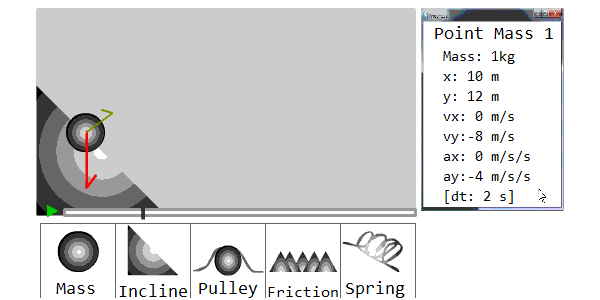
\includegraphics[width=0.8\textwidth]{img/concept}}
    \caption{Concept for interactive sandbox}
\end{figure}

\clearpage
\BgThispage
Once the components are in place, users can select play and the canvas will come to life. The components will move over time according to their properties, allowing students to visualize the system. At any point, users can pause the simulation and select a component to view its properties, allowing them to get quantitative results in addition to the visualization. We believe that by combining animated graphics with numeric descriptions, students will be able to develop an intuition for what kind of behaviors are associated with otherwise incomprehensible equations and formulas.

Though the sandbox is the core feature and an ambitious project in its own right, it is far from Principia's only selling point. To enable users to connect with and support one another, the website will allow them to create accounts. A registered user can save and load his creations, share them with others, browse simulations, provide comments and annotations, and even create quizzes or walkthroughs. Imagine a future where instructors integrate Principia into their course. No longer will students work in isolation, writing out equations based on a fixed image or an ambiguous word problem. Instead, students will have the chance to have a dialogue with both the instructor and their peers, exploring problems interactively or even inventing their own systems.

We see the final version of our project as a top site for physics education and a powerful supplement to material covered in the classroom. Teachers, students, and the growing community of individuals interested in online learning at their own pace will all be able to take advantage of Principia.